\documentclass[aspectratio=169]{beamer}
\usepackage{tikz}
\usepackage{graphicx}
\usepackage{listings}
\usepackage{xcolor}
\usepackage{hyperref}
\usepackage[spanish,es-noquoting]{babel}
\usepackage[round]{natbib}

\lstset{
  basicstyle=\ttfamily\small,
  keywordstyle=\color{blue},
  stringstyle=\color{red},
  commentstyle=\color{gray},
  showstringspaces=false
}

% Clean Theme Setup & Optimization
\usetheme{Warsaw}
\usecolortheme{default}
\usefonttheme{serif}

% Remove top headline bar and navigation clutter to maximize slide text space
\setbeamertemplate{headline}{}
\setbeamertemplate{navigation symbols}{}
\setbeamertemplate{frametitle continuation}{}

% Slim, clean footline bar
\setbeamertemplate{footline}{
  \leavevmode%
  \hbox{%
    \begin{beamercolorbox}[wd=.333333\paperwidth,ht=2.25ex,dp=1ex,left]{author in head/foot}%
      \hspace*{2ex}\insertshortauthor
    \end{beamercolorbox}%
    \begin{beamercolorbox}[wd=.333333\paperwidth,ht=2.25ex,dp=1ex,center]{title in head/foot}%
      \insertshorttitle
    \end{beamercolorbox}%
    \begin{beamercolorbox}[wd=.333333\paperwidth,ht=2.25ex,dp=1ex,right]{date in head/foot}%
      \insertframenumber{} / \inserttotalframenumber\hspace*{2ex}
    \end{beamercolorbox}%
  }%
  \vskip0pt%
}

% Font size and list spacing optimizations to prevent text overflow
\setbeamertemplate{itemize/enumerate body begin}{\small}
\setbeamertemplate{itemize/enumerate subbody begin}{\footnotesize}
\setbeamertemplate{itemize/enumerate subsubbody begin}{\scriptsize}

\makeatletter
\g@addto@macro\itemize{%
  \setlength{\itemsep}{2pt}%
  \setlength{\parsep}{1pt}%
  \setlength{\topsep}{2pt}%
  \setlength{\partopsep}{0pt}%
}
\makeatother

\graphicspath{{../}{./}}
\setbeamertemplate{caption}[numbered]

% Title info
\title[Módulo 3]{Módulo 3}
\subtitle{ Convertir conocimiento individual en capacidad institucional}
\author{Ricardo Reyes-Jimenez}
\institute{Universidad de La Sabana}
\date{\today}


% Background image for title slide
\usebackgroundtemplate{
  \tikz\node[opacity=0.3]{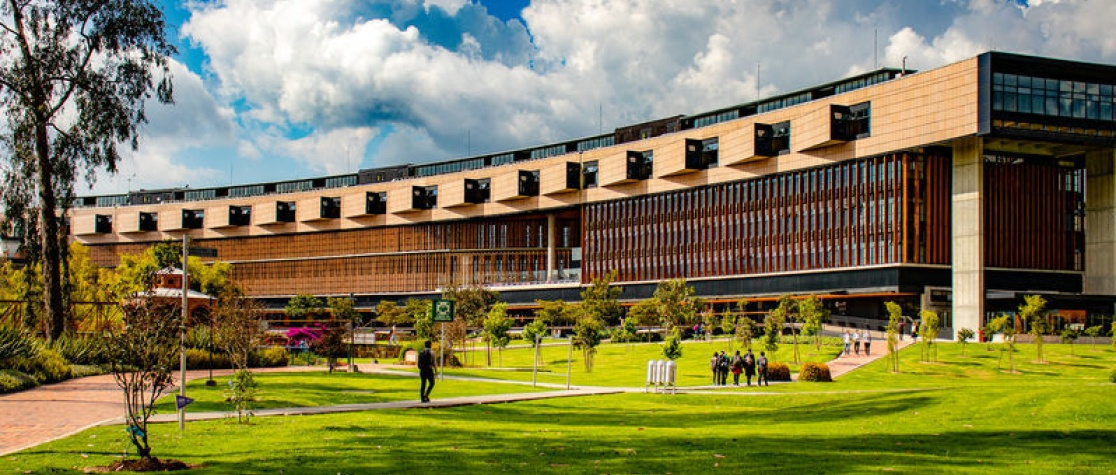
\includegraphics[width=\paperwidth,height=\paperheight]{Images/UniSabana.jpg}};
}


\begin{document}

% Title slide
\begin{frame}
  \titlepage
\end{frame}

% Reset background for normal slides
\usebackgroundtemplate{}


\begin{frame}[allowframebreaks,fragile]{Objetivos de la Sesión}


Al finalizar esta sesión serás capaz de:

\begin{itemize}
  \item Comprender qué es una PromptLibrary.
  \item Identificar oportunidades de reutilización.
  \item Diseñar Blueprints jurídicos reutilizables.
  \item Documentar prompts de alto valor.
  \item Reducir la pérdida de conocimiento organizacional.
\end{itemize}
\end{frame}

\begin{frame}[allowframebreaks,fragile]{La Paradoja de la IA Jurídica}


Nunca ha sido tan fácil acceder a IA.

Sin embargo:

\begin{itemize}
  \item Miles de horas de aprendizaje se desperdician.
  \item Los abogados trabajan de forma aislada.
  \item Los mejores prompts rara vez se documentan.
  \item Cada persona reinventa soluciones ya descubiertas.
\end{itemize}
\end{frame}

\begin{frame}[allowframebreaks,fragile]{El Coste Oculto del Trabajo Repetitivo}


¿Cuántas veces en un mes realizas?

\begin{itemize}
  \item Resúmenes de expedientes.
  \item Revisión de contratos.
  \item Elaboración de conceptos.
  \item Búsqueda jurisprudencial.
  \item Matrices de riesgos.
\end{itemize}
La IA puede acelerar estas tareas.

La pregunta no es \textit{si puede hacerlo}.

La pregunta es \textit{cómo hacerlo de forma consistente}.

\end{frame}

\begin{frame}[allowframebreaks,fragile]{El Problema de los Silos de Conocimiento}


Cuando un abogado desarrolla un prompt excelente:

\begin{itemize}
  \item Obtiene mejores resultados.
  \item Ahorra tiempo.
  \item Mejora la calidad.
\end{itemize}
Pero si no lo documenta:

\begin{itemize}
  \item El conocimiento desaparece.
  \item Nadie más aprende.
  \item La organización no mejora.
\end{itemize}
\end{frame}

\begin{frame}[allowframebreaks,fragile]{¿Qué es una PromptLibrary?}


Una PromptLibrary es:

> Un repositorio organizado de instrucciones probadas y reutilizables para interactuar con sistemas de IA.

No es una colección de trucos.

Es infraestructura de conocimiento.

\end{frame}

\begin{frame}[allowframebreaks,fragile]{Analogía Jurídica}


Una firma jurídica ya dispone de:

\begin{itemize}
  \item Modelos de contratos.
  \item Plantillas de demandas.
  \item Minutas.
  \item Conceptos de referencia.
\end{itemize}
La PromptLibrary cumple la misma función para la IA.

\end{frame}

\begin{frame}[allowframebreaks,fragile]{ROI Individual vs ROI Institucional}


Uso individual:

\begin{itemize}
  \item Un abogado mejora.
\end{itemize}
Uso institucional:

\begin{itemize}
  \item Cien abogados mejoran.
\end{itemize}
La verdadera transformación ocurre cuando el conocimiento se comparte.

\end{frame}

\begin{frame}[allowframebreaks,fragile]{Ciclo de Pérdida de Conocimiento}


\begin{itemize}
  \item Se descubre un buen prompt.
  \item Se utiliza exitosamente.
  \item El usuario cierra la ventana.
  \item Nadie documenta nada.
  \item El aprendizaje desaparece.
\end{itemize}
Este ciclo se repite diariamente.

\end{frame}

\begin{frame}[allowframebreaks,fragile]{Anatomía de una PromptLibrary Moderna}


Debe contener:

\begin{itemize}
  \item Nombre.
  \item Objetivo.
  \item Área jurídica.
  \item Blueprint.
  \item Ejemplos.
  \item Fecha.
  \item Responsable.
  \item Observaciones.
\end{itemize}
\end{frame}

\begin{frame}[allowframebreaks,fragile]{¿Qué es un Blueprint?}


Un Blueprint es una plantilla parametrizable.

No contiene un caso específico.

Contiene una estructura reutilizable.

\end{frame}

\begin{frame}[allowframebreaks,fragile]{Ejemplo Simple de Blueprint}


Prompt tradicional:

``Resume este contrato.''

Blueprint:

``Actúa como abogado senior especializado en [ÁREA]. Resume el siguiente [TIPO DE DOCUMENTO] identificando [ELEMENTOS CLAVE].''

\end{frame}

\begin{frame}[allowframebreaks,fragile]{El Poder de las Variables}


Variables frecuentes:

\begin{itemize}
  \item [TIPO DE CONTRATO]
  \item [JURISDICCIÓN]
  \item [TIPO DE PROCESO]
  \item [ROL DEL CLIENTE]
  \item [DOCUMENTO]
\end{itemize}
Las variables permiten reutilización.

\end{frame}

\begin{frame}[allowframebreaks,fragile]{Restricciones: El Componente Más Olvidado}


Toda IA necesita límites.

Ejemplos:

\begin{itemize}
  \item No inventes información.
  \item Cita textualmente.
  \item Utiliza tabla.
  \item Limita la respuesta a 500 palabras.
\end{itemize}
\end{frame}

\begin{frame}[allowframebreaks,fragile]{Caso Práctico: Análisis de Sentencias}


Objetivo:

Extraer:

\begin{itemize}
  \item Hechos.
  \item Problema jurídico.
  \item Regla jurídica.
  \item Decisión.
  \item Salvamentos de voto.
\end{itemize}
Resultado:

Una ficha jurisprudencial consistente.

\end{frame}

\begin{frame}[allowframebreaks,fragile]{Caso Práctico: Revisión Contractual}


Objetivo:

Detectar:

\begin{itemize}
  \item Penalidades.
  \item Exclusividad.
  \item Terminación anticipada.
  \item Limitaciones de responsabilidad.
\end{itemize}
La IA debe funcionar como primera capa de revisión.

\end{frame}

\begin{frame}[allowframebreaks,fragile]{Caso Práctico: Litigio}


Blueprint enfocado en:

\begin{itemize}
  \item Cronologías.
  \item Contradicciones.
  \item Teorías del caso.
  \item Riesgos probatorios.
\end{itemize}
\end{frame}

\begin{frame}[allowframebreaks,fragile]{Caso Práctico: Contratación Estatal}


Aplicaciones:

\begin{itemize}
  \item Revisión de pliegos.
  \item Verificación documental.
  \item Matrices de cumplimiento.
  \item Identificación de riesgos.
\end{itemize}
\end{frame}

\begin{frame}[allowframebreaks,fragile]{Principales Errores al Diseñar Prompts}


Error 1: Ambigüedad.

Error 2: Falta de contexto.

Error 3: Falta de restricciones.

Error 4: Objetivos mal definidos.

\end{frame}

\begin{frame}[allowframebreaks,fragile]{Calidad Jurídica}


La IA no reemplaza criterio profesional.

Siempre debe existir:

\begin{itemize}
  \item Revisión humana.
  \item Validación jurídica.
  \item Control de calidad.
\end{itemize}
La responsabilidad profesional sigue siendo humana.

\end{frame}

\begin{frame}[allowframebreaks,fragile]{Riesgos Jurídicos}


Riesgos frecuentes:

\begin{itemize}
  \item Alucinaciones.
  \item Sesgos.
  \item Respuestas desactualizadas.
  \item Interpretaciones incorrectas.
\end{itemize}
\end{frame}

\begin{frame}[allowframebreaks,fragile]{Protección de Información}


Nunca debe compartirse:

\begin{itemize}
  \item Información protegida por secreto
\end{itemize}
\end{frame}



\begin{frame}[allowframebreaks]{References}
  \bibliographystyle{apalike}
  \bibliography{references}
\end{frame}


\end{document}